\section{Zasady SOLID}

\subsection{SRP - Zasada pojedynczej odpowiedzialności (ang. \textbf{S}OLID)}

Zasada mówi, że każdy moduł, zestaw, klasa czy metoda powinna posiadać pojedynczy obszar odpowiedzialności (przyczynę zmian).  W momencie zmian wymagań, określa się jakie klasy są odpowiedzialne za dane wymagania i to te kasy się modyfikuje. Jeśli istnieją co najmniej dwa niezależne powody mogące wymusić zmianę w danej klasie, to dana klasa rozciąga się na więcej niż jeden obszar odpowiedzialności. W przypadku naruszenia zasady SRP zmiany w dwóch różnych wymaganiach implikują modyfikację w jednej, tej samej klasie. 

\begin{tcolorbox}[colback=yellow]	
	\textbf{Zasada pojedynczej odpowiedzialności}\\
	Żadna klasa nie może być modyfikowana z więcej niż jednego powodu.
\end{tcolorbox}


Wyobraźmy sobie sytuację, w której klasa rysująca figurę geometryczną na ekranie jest odpowiedzialna zarówno za wspomniane rysowanie, ale również za wyznaczanie pola powierzchni danej figury np. \texttt{Rectangle}. Jakie konsekwencje to za sobą niesie? Jeśli dwa zestawy np. GUI oraz jakiś inny korzystający jedynie z operacji liczenia pola powierzchni będą związane z klasą \texttt{Rectangle} to zmiana wynikająca z wymagań związanych z GUI może pociągać ryzyko nieprawidłowego działania w drugim zestawie. Chcąc zachować zasadę SRP należałoby stworzyć dwie osobne klasy: jedną rysująca figurę i drugą liczącą pole powierzchni. Pierwsza z nich może wykorzystywać tę pierwszą. 

Oczywiście należy zawsze mieć na uwadze, że rozdrabniać klasy na coraz mniejsze typy można tak długo, aż zbyt dużego skomplikowania projektu. Konieczne jest branie pod uwagę wymagań i ich potencjalnych zmian.

Przeanalizujmy interfejs \texttt{IModem}.
\begin{lstlisting}[caption={Naruszenie zasady SRP}, label={lab1/lst/srpViolationModem}]
	public interface Modem
	{
		public void Dial(string phoneNumber);
		public void Hangup();
		public void Send(char c);
		public char Recieve();
	}
\end{lstlisting}
Tutaj konieczne jest przeanalizowanie wymagań, ponieważ podział interfejsu na dwa zawierające odpowiednio Dial i Hangup oraz Send i Recieve może być nie potrzebne, jeśli zmiany w aplikacji nie wpływają na zmiany w metodach zarządzających wykonywaniem połączeń.

\subsubsection{Zadanie 1}
\begin{lstlisting}[caption={Naruszenie zasady SRP}, label={lab1/lst/srpViolationEmployee}]
class Employee()
{
	public void CalculatePay();
	public void Store();
}
\end{lstlisting}
W powyższym przykładzie została naruszona zasada SRP, zaproponuj sposób rozdzielenia odpowiedzialności tej klasy. 




\subsection{OCP - Zasada otwarte - zamknięte (ang. S\textbf{O}LID)}

Pisząc elastyczny kod powinniśmy być w stanie wprowadzać nowe funkcjonalności dodając nowe klasy i w tym samym momencie \textbf{nie} modyfikując tych już istniejących. Nie zawsze jest to możliwe, ale warto próbować. 

\begin{tcolorbox}[colback=yellow]	
\textbf{Zasada otwarte - zamknięte}\\
Składniki oprogramowania (klasy, moduły, funkcje itp.) powinny być otwarte na rozbudowę, ale zamknięte dla modyfikacji.
\end{tcolorbox}

Aby osiągnąć ten cel oprogramowanie powinno posiadać jasno zdefiniowane, niezmienne abstrakcje. Jeśli dany moduł wykorzystuje jedynie abstrakcje, nie powinna być konieczna jego modyfikacja w przypadku zmian wymagań, rozszerzania funkcjonalności. Stosowanie zasady OCP wymaga wykorzystania polimorfizmu.

Przeanalizujmy poniższy diagram UML. W tym przypadku zmiana obiektu \texttt{Order} wymagała by zmian w klasie klienta. 

\begin{figure}[hbt!]
	\centering
	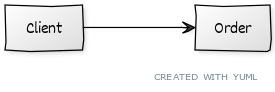
\includegraphics[width=0.6\linewidth]{images/SolidOcpViolationUml}
	\caption{Diagram UML, gdzie \texttt{Client} narusza zasadę OCP.}
	\label{lab1/fig/SolidOcpViolationUml}
\end{figure}
%[Client]->[Order]
%[Client]
%[Order]

Stosując wzorzec projektowy strategia, który zostanie omówiony na kolejnych zajęciach mamy możliwość odwrócenia zależności. Jeśli w wyniku rozszerzania, zmian funkcjonalności okaże się, że klasa Order powinna zostać zmieniona, będzie można utworzyć nową wersję klasy implementującej interfejs zdefiniowany przez klienta i ją podmienić bez modyfikacji w samej klasie \texttt{Client}.

%Zastosowano interfejs IClient zamiast IOrder, ponieważ związki klas abstrakcyjnych z klasami klienckimi są ściślejsze niż z konkretnymi potomnymi, które je implementują. 
\begin{figure}[hbt!]
	\centering
	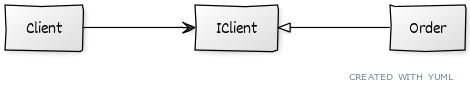
\includegraphics[width=0.9\linewidth]{images/SolidOcpUml}
	\caption{Diagram UML, gdzie \texttt{Client} \textbf{nie} narusza zasady OCP.}
	\label{lab1/fig/SolidOcpUml}
\end{figure}
%[Client]->[IClient]^[Order]
%[Client]
%[IClient]
%[Order]

Wyobraźmy sobie moduł odpowiedzialny za rysowanie figur geometrycznych. Parametrem tej metody jest lista obiektów. Jeśli w wyniku zmian konieczne okaże się dodanie nowej klasy np. \texttt{Diamond} wymagane będą zmiany w klasie \texttt{Drawer}.
\begin{lstlisting}[caption={Naruszenie zasady OCP}, label={lab1/lst/ocpViolationShapes}]
public class Circle { }
public class Square { }

public static class Drawer {
	public static void DrawShapes(IEnumerable<object> shapes) {
		foreach (object shape in shapes) {
			if (shape is Circle) {
				(shape as Circle).DrawCircle();
			} else if (shape is Square) {
				(shape as Square).DrawSquare();
			}
		}
	}
}
\end{lstlisting}

Stosując polimorfizm i abstrakcję możemy uniezależnić klasę \texttt{Drowe} od konkretnych typów. Dzięki utworzeniu wspólnego interfejsu i przekazywanie listy obiektów implementujących ten interfejs, dodanie nowej figury nie będzie wymagało zmian w kodzie klienta. Nie musimy dostosowywać już istniejące kodu do zmian.

\begin{lstlisting}[caption={Naruszenie zasady OCP}, label={lab1/lst/ocpViolationShapes}]
public interface IShape { void Draw(); }
public class Circle : IShape { public void Draw() { }}
public class Square : IShape { public void Draw() { } }

public static class Drawer {
	public static void DrawShapes(IEnumerable<IShape> shapes) {
		foreach (IShape shape in shapes) {
			shape.Draw();
		}
	}
}
\end{lstlisting}

%Niestety istnieją takie zmiany, na które powyżej pokazana implementacja nie jest odporna np. jeśli kolejność rysowania figur okazałaby się konieczna do uwzględnienia. To projektant musi przewidzieć jakie zmiany są najbardziej prawdopodobne i określić odpowiednie zabezpieczenia. Zamiast stosować punkty szczepień (miejsca w programie, w których przewidujemy, że być może kiedyś będą zmiany), może zastosować zasadę mówiącą, że "Gdy raz mnie oszukasz, powinieneś się wstydzić. Kiedy oszukasz mnie po raz drugi, to ja powinienem się wstydzić". Jednocześnie powinniśmy na bieżąco sprawdzać nasze oprogramowanie i zdobywać wiedzę o prawdopodobnych rodzajach zmian. 

%Problem z kolejnością rysowanych figur możnaby rozwiązać stosując dodatkową klasę ShapeComparer : IComparer, która to zawiera statyczną tablicę priorytetów, na której to podstawie określane są priorytety rysowania figur. Metoda DrawShapes może wtedy wywolać metodę shapes.Sort(new ShapeComparer) prze rysowaniem figur (str. 186).

Oczywiście zmiany będą również konieczne w module, który tworzy instancje obiektów typu \texttt{Shape}. Ale ten proces jest zazwyczaj hermetyzowany w metodzie \texttt{Main}, albo np. w klasie fabryki abstrakcyjnej. 

\subsection{LSP - Zasada podstawienia Liskov (ang. SO\textbf{L}ID)}

Zasada podstawienia Liskov pozawala odpowiedzieć na pytanie jakie są dobre praktyki tworzenia hierarchii klas i co zrobić, aby były one zgodne z zasadą otwarte-zamknięte. W sytuacji braku możliwości podstawienia obiektów pochodnych w miejsce obiektów klasy bazowej występuje naruszenie zasady LSP. Często w konsekwencji zostaje również naruszona zasada OCP.

\begin{tcolorbox}[colback=yellow]	
\textbf{Zasada podstawienia Liskov}\\
Musi istnieć możliwość zastępowania typów bazowych ich podtypami.
\end{tcolorbox}

Lepsze zrozumienie zasady LSP można uzyskać analizując popularny przykład z klasą prostokąta oraz klasą pochodną kwadratu. Zasadność stosowania dziedziczenia często jest analizowania przez zadanie sobie pytania czy klasy są w relacji \textbf{IS-A}. Niewątpliwie kwadrat jest prostokątem. Jednak pierwszy problem się pojawia w sytuacji, gdy chcemy zaimplementować/skorzystać z właściwości \texttt{Height} oraz \texttt{Width}. Są one całkowicie sensowne w przypadku prostokąta, jednak wątpliwe w klasie kwadratu. 

Idąc dalej można napisać klasę tak, że w momencie ustawiania właściwości wysokości albo szerokość w klasie kwadratu, będzie ustawiana zarówno wysokości jak i szerokość na taką samą wartość. Właściwości te mogą w klasie bazowej mogą być wirtualne. Dodatkowo zakładamy, że w obu klasach została zaimplementowana metoda \texttt{Area()}, zwracająca pole powierzchni danej figury.

Spójrzmy na poniższy kod, w sytuacji gdy do funkcji zostałby przekazany obiekt kwadratu.
\begin{lstlisting}[caption={Naruszenie zasady LSP}, label={lab1/lst/lspViolationSquareRectangle}]
void Foo(Rectangle r)
{
	r.Width = 5;
	r.Height = 4;
	if(r.Area() != 20) {throw new ...}
}
\end{lstlisting}

W powyższym przypadku okazuje się, że klient nie jest w stanie użyć instancji klasy pochodnej, w miejscu, gdzie oczekuje klasy bazowej. Autor klasy pochodnej naruszył niezmienność klasy bazowej \texttt{Rectangle}.


Przewidzieć takie założenia, można za pomocą  programowanie przez kontrakt (tzw. DBC ang. Design By Contract). Polega ona na dodaniu do metod pewnych warunków wejściowych oraz wyjściowych, które muszą być spełnione, aby metoda mogła się wykonać. 

\begin{tcolorbox}[colback=yellow]	
Ponowna deklaracja procedury (w klasie potomnej) może zastępować warunki wstępne tylko warunkami równymi lub słabszymi, natomiast warunki wyjściowe może zastępować tylko warunkami równymi lub mocniejszymi.
\end{tcolorbox}

Warunki wyjściowe właściwości \texttt{Rectangle.Width} mogłyby zostać zdefiniowane jako:
\begin{lstlisting}
	assert((width ==w) && (height == old.height));
\end{lstlisting}

Innym problemem, może być sytuacja, gdy dana metoda klasy bazowej przyjmuje dowolny obiekt, natomiast w klasie pochodnej istnieje nieznany wymóg, że obiekt ten musi być konkretnego typu np. z powodu wykonywania operacji rzutowania. Klasa pochodna będzie zgłaszać niezrozumiały dla klienta wyjątek.

\subsection{ISP - Zasada segregacji interfejsów (ang. SOL\textbf{I}D)}

Interfejsy klas nie powinny być zbyt rozbudowany. Jeżeli jedna klasa korzysta jedynie w pewnych funkcjonalności jakie zakłada interfejs, a druga z innych to taki interfejs powinien zostać podzielony na dwa niezależne od siebie. Do celów zapewnienia zgodności z zasadą separacji interfejsów można skorzystać z techniki dziedziczenia wielokrotnego. Należy pamiętać, że w C\# klasa nie może dziedziczyć po więcej niż jeden klasie, natomiast może implementować wiele interfejsów. Obiekty klienckie mogą korzystać z tego samego obiektu za pośrednictwem różnych interfejsów. Powinny one zależeć wyłącznie od wywoływanych przez siebie metod.  

\begin{tcolorbox}[colback=yellow]	
	\textbf{Zasada segregacji interfejsów}\\
	Klient nie powinien być zmuszany do zależności od metod, których nie używa.
\end{tcolorbox}


Wyobraźmy sobie, że musimy przygotować program obsługujący interfejs użytkownika bankomatu. Konieczne jest zapewnienie możliwości obsługi urządzenia w wykorzystaniem interfejsu graficznego, syntezatora mowy oraz za pomocą języka Braille'a. 

Zakładamy, że każda operacja dowolnej transakcji jest realizowana przez osobną klasę na przykład mogą to być typy: \texttt{DepositTransaction}, \texttt{WithdrowalTransaction} oraz \texttt{TransferTransaction}, wszystkie mogą dziedziczyć po abstrakcyjnej klasie bazowej. Jednocześnie wszystkie muszą korzystać z klas, które realizują funkcję UI i implementują interfejs UI. Klasa realizująca obsługę z wykorzystaniem syntezatora mowy, musi implementować wszystkie może operacje przewidziane przez klasy pochodne względem \texttt{Transaction}, co jest sensowne. Problemem jest jednak fakt, że np. klasa \texttt{DepositTransaction} musi niepotrzebnie znać/posiadać referencje do całego obiektu implementującego UI. Wystarczyłaby by funkcja \texttt{RequestDepositAmount}, obiekt nie jest zainteresowany np. \texttt{RequestTransferAmount}. 

Rozwiązanie tego problemu zostało pokazano na diagramie UML~\ref{lab1/fig/SolidIspUml}. Dzieląc gruby interfejs \texttt{IUI} można odciążyć klientów od posiadania referencji od obiektów, których funkcjonalności nie potrzebują. Co więcej, jeśli zostanie dodana nowa transakcja np. \texttt{PayGasBillTransaction} nie będzie konieczności ponownej przebudowy pozostałych klas transakcji w wyniki zmiany grubego interfejsu UI. 

\begin{figure}[hbt!]
	\centering
	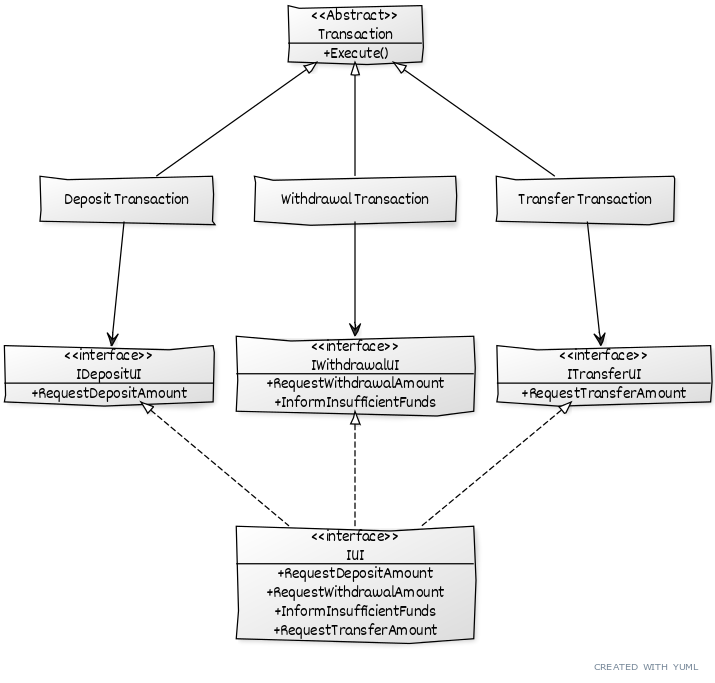
\includegraphics[width=0.8\linewidth]{images/SolidIspUml}
	\caption{Diagram UML projektu w którym zrealizowano zasadę segregacji interfejsów.}
	\label{lab1/fig/SolidIspUml}
\end{figure}
%[Transaction]^[Deposit Transaction]
%[Transaction]^[Withdrawal Transaction]
%[Transaction]^[Transfer Transaction]
%
%[Deposit Transaction]->[DepositUI]
%[Withdrawal Transaction]->[WithdrawalUI]
%[Transfer Transaction]->[TransferUI]
%
%[DepositUI]^-.-[UI]
%[WithdrawalUI]^-.-[UI]
%[TransferUI]^-.-[UI]
%
%[<<Abstract>>Transaction|+Execute()]
%
%[Deposit Transaction]
%[Withdrawal Transaction]
%[Transfer Transaction]
%
%[≪interface≫;DepositUI|+RequestDepositAmount]
%[≪interface≫;WithdrawalUI|+RequestWithdrawalAmount;+InformInsufficientFunds]
%[≪interface≫;TransferUI|+RequestTransferAmount]
%
%[≪interface≫;UI|+RequestDepositAmount;+RequestWithdrawalAmount;+InformInsufficientFunds;+RequestTransferAmount]

W sytuacji, gdy pewna klasa kliencka albo metoda, potrzebowałaby wykorzystać obiekt implementujący zarówno \texttt{IDepositUI} oraz \texttt{IWithdrowalUI}, można jako argumenty konstruktora i metody przekazać dwa razy ten sam obiekt w następujący sposób: \texttt{void Foo(IDepositUI depositUI, IWithdrowalUI withdrowalUi)} i~wywołując funkcję: Foo(ui,ui).




\subsection{DIP - Zasada odwracania zależności (ang. SOLD)}

Głównie za sposób działania aplikacji odpowiadają moduły wysokopoziomowe. To one zawierają logikę biznesową, która często jest wielokrotnie wykorzystywana. Przemyślana architektura obiektowa powinna składać się z wyraźnie zdefiniowanych i odznaczających się warstw. Usługi powinny być opisane odpowiednimi, niezmiennymi interfejsami.

\begin{tcolorbox}[colback=yellow]	
	\textbf{Zasada odwracania zależności}\\
	A. Moduły wysokopoziomowe nie powinny zależeć od modułów niskopoziomowych. Obie grupy modułów powinny zależeć od abstrakcji.\\
	B. Abstrakcje nie powinny zależeć od szczegółowych rozwiązań. To szczegółowe rozwiązania powinny zależeć od abstrakcji.
\end{tcolorbox}

Nie należy postrzegać bibliotek jako właścicieli interfejsów. Interfejsy powinny być powiązane ze swoimi właścicielami i klasy z innej warstwy powinny implementować te interfejsy. Pozwala to tworzyć oprogramowanie, które jest elastyczne. Jeśli dany zestaw jest wykorzystywany przez kilku klientów np. pobrany pakiet NuGet to warto stworzyć dodatkową warstwę abstrakcji, która umożliwi w przyszłości zmianę tego pakietu, bez konieczności wprowadzania zmian po stronie klienta. Można to osiągnąć np. stosując wzorzec projektowy adapter, który zostanie omówiony na przyszłych zajęciach. Oczywiście jeśli mamy do czynienia z klasami, które są zmieniane bardzo rzadko, albo mamy wysoki poziom zaufania to autorów to uzależnienie się od nich nie jest czymś złym. Ciężko znaleźć sens, tworzenia dodatkowej warstwy pośredniej do komunikowania się z klasą \texttt{string}.

Wyobraźmy sobie przykład dwóch klas \texttt{Button} oraz \texttt{Lamp}. Klasa przycisku ma możliwość sterowania lampą. W najprostszej, naiwnej implementacji można by dodać pole w klasie \texttt{Button} przechowujące referencje do obiektu lampy. \texttt{Lamp} mógłby być przekazywany np. jako argument konstruktora. Co jest w tym podejściu złe? Czy przycisk może sterować innymi urządzeniami? \texttt{Button} będący wysokopoziomową abstrakcją, jest uzależniony od niskopoziomowego obiektu lampy.

Powyższy problem można by rozwiązać przez dodanie interfejsu np. \texttt{SwitchableDevice} i wstrzykiwanie obiektu go implementującego do obiektu \texttt{Button}. Teraz wystarczy, aby \texttt{Lamp} implementował ten interfejs. W przypadku, kiedy przycisk będzie miał zostać wykorzystany do sterowania np. silnikiem albo piecem wystarczy utworzyć nowy obiekt \texttt{Motor} albo \texttt{Heater}, który będzie implementował \texttt{SwitchableDevice} i przekazać go do obiektu \texttt{Button}.

\subsubsection{Zadanie 1}
Przeanalizuj poniższy kod i zmień go tak, aby był zgodny z omawianą zasadą DIP.
\begin{lstlisting}
const byte THERMOMETER = 0X86;
const byte FURNACE = 0X87;
const byte ENGAGE = 1;
const byte DISENGAGE = 0;

void Regulate(double minTemp, double maxTemp)
{
	for(;;)
	{
		while (in(THERMOMETER) > minTemp){ wait(1); }
		out(FURNACE, ENGAGE);
		while (in(THERMOMETER) < maxTemp){ wait(1); }
		out(FURNACE, DISENGAGE);	
	}
}
\end{lstlisting}

Możesz utworzyć dwa dodatkowe interfejsy, jeden dla obiektów mierzących temperaturę i drugi dla obiektów odpowiedzialnych za zmianę temperatury np. pieców. Dalej utwórz dwie konkretne klasy np \texttt{Thermometer} oraz \texttt{Heater} i uzależnij obiekt regulacji od tych abstrakcji. 